%\section*{Summary}
\chapter{Decisions in a riskless world\clabel{Riskless}}
%Decision theory is re-developed. How should an individual decide whether to take some gamble (the usual way of phrasing decision problems in economics)? We solve typical decision problems (gamble evaluation) by considering the time-average growth rate (or the [time- and ensemble-] average of the ergodic growth rate) under multiplicative dynamics. The construction of an ergodic observable motivates the introduction of a non-linear function that encodes the dynamics. This function is historically called the “utility function” and encodes the dynamics. 
%
%In life we frequently find ourselves in situations which require us to make decisions, \ie to choose between two or more available actions whose outcomes may be uncertain. In this lecture we shall develop a theory of how individuals make such decisions. Of course, this is far too broad a promise. We can't possibly develop a {\it complete} theory of decisions in a single lecture, and perhaps not even in a lifetime. Indeed, since we will be studying mathematical models of decisions, we will necessarily have little to say about actions whose outcomes cannot be quantified, \eg in pounds, shillings, and pence. This lecture will not tell you whom you should marry or even whose economics lectures you should attend.
%
%Instead, we will narrow our gaze to problems which are mathematically tractable but, we hope, no less illuminating for being so. Specifically we will solve the gamble problem, which is the canonical problem in decision theory. Its treatment forms the cornerstone on which much of classical economics -- such as utility theory, game theory, and asset pricing -- is built.

%We shall not consider whether our theory is prescriptive, in that it informs us how individuals {\it should} make decisions, or descriptive, in that informs us how they {\it do}. This is an important epistemological question in decision theory but, for now at least, we will leave it to the philosophers.

{\it Decision theory is a cornerstone of formal economics. As the name suggests, it 
models how people make decisions. In this chapter we will generalise and formalise
the treatment of the coin tossing game to introduce our 
approach to decision theory. Our central axiom will be that people attempt to maximize
the rate at which wealth grows when averaged over time. This is a surprisingly powerful idea.
In many cases it eliminates the need for well established but epistemologically troublesome techniques, such as utility functions. 
}
\newpage

\section{Models and science fiction}
\seclabel{Models_and}
We will do decision theory 
by using mathematical models, and since this can be done in many ways we will be
explicit about how we choose to do it. We will define a wealth process -- a model of how wealth changes with time -- 
and a decision criterion. The wealth process and the decision criterion may or may not remind you
of the real world. We will not worry too much about the accuracy 
of these reminiscences. Instead we will ``shut up and calculate'' -- we will let the mathematical
model create its world. Writing down a mathematical model is like laying out the premise for
a science-fiction novel. We may decide that people can download their consciousness onto a computer, 
that medicine has advanced to eliminate ageing and death -- these are premises we are at liberty to invent.
Once we have written them down we begin to explore the world that results from those premises.
A decision criterion is really a model of human behaviour -- what makes us who we are if not our decisions? 
It therefore implies a long list of specific behaviours that will
be observed in a given model world. For example, some criteria will lead to cooperation, others will not, some will lead
to the existence of insurance contracts, others will not \etc We will explore the worlds created by the different
models. Once we have done so we invite you to judge which model you find most useful
for your understanding of the world. Of course, having spent many years thinking about these
issues we have come to our own conclusions, and we will put them forward because we believe them to be helpful.

To keep the discussion to a manageable volume we will only consider a setup that corresponds to
making purely financial decisions. We may bet on a horse or take out personal liability insurance.
This chapter will not tell you whom you should marry or even whose economics lectures you should attend.

%%%%%%%%%%%%%%%%%%%%%%%%%%%%%%%%%%%%%%%%%%%%%%%

%%%%%%%%%%%%%%%%%%%%%%%%%%%%%%%%%%%%%%%%%%%%%%%
\section{The decision axiom}

A ``decision theory'' is a model of human behaviour. We will write down such a model phrased as the following simple 
axiom: 

\begin{keypts}{Decision axiom}

People optimize the growth rate of their wealth.

\end{keypts}

Without discussing why people might do this, let's step into the world created by this axiom. To do that, we need to be crystal clear about what a growth rate is, so we'll discuss that first, in \secref{Growth_rates}. Traditionally, decision theory deals with an uncertain future: we have to decide on
a course of action now although we don't know with certainty what will happen to us in the future under any
of our choices. We will systematically work our way towards this setup, beginning with trivial decisions where neither time nor uncertainty matters \secref{Different_magnitudes}, next introducing time \secref{Different_magnitudes_and} (where we will recover what's called ``discounting''), and finally working with both time and uncertainty \secref{Decisions_in_an} (where we will recover ``expected utility theory'').

%
\section{Growth rates\seclabel{Growth_rates}}

You may have wondered why both 
\be
\gad=\frac{\x(\t+\Dt)- \x(\t)}{\Dt}
\elabel{add_rate}
\ee
 and 
\be
\gexp= \frac{\ln \x(\t+\Dt)-\ln \x(\t)}{\Dt}
\elabel{exp_rate}
\ee
are sometimes called a growth rate -- they're different objects, why the same name? By the end of this section, the answer to this question should be clear.

When we say that $\x(\t)$ is a growth process, we mean that it is a monotonic function of $\t$. If you're thinking about randomness -- don't, we'll come to that later. For now, we will just work with a deterministic function $\x(\t)$.

For a given process, the appropriate growth rate, $\g$, solves the following problem for us: how do we characterise how fast $\x$ grows?
A growth rate is a mathematical object of the form
\be
\g=\frac{\D\gv(\x)}{\Dt},
\elabel{gen_rate}
\ee
were $\gv(\x)$ is a monotonically increasing function of wealth $\x$. Comparing to \eref{add_rate} and \eref{exp_rate}, we find that $\gv(\x)=\x$ for additive dynamics and $\gv(\x)=\ln \x$ for multiplicative dynamics. The transformation $\x \to \gv(\x)$ ensures temporal stability of $\g$.

How does this work, and what does it mean? Specifically, 
\bi
\item[1.]
why the transformation? 
\item[2.]
how do we know which transformation to use?
\ei
We will start with the mathematically simple case of the additive growth rate, \eref{add_rate}, and discuss its properties by applying it to additive growth. Next we will ask under what conditions the exponential growth rate, \eref{exp_rate}, is appropriate, and that will lead us to the general growth rate, \eref{gen_rate}.

%$\x(\t)$ grows according to some dynamic, meaning it is some function. In order to say meaningfully at what rate $\x$ is growing, this rate has to be stable in time. For example, if $\x(\t)$ grows exponentially, the additive rate of change $\frac{\D\x}{\Dt}$ will change throughout time. 

\subsection{Additive growth rate\seclabel{add_rate}}
If I want to know how fast $\x(\t)$ grows, the most obvious thing to compute is its rate of change -- that's the additive growth rate, \eref{add_rate}.
This tells me by how much $\x$ grows in the interval $[\t,\t+\Dt]$. If $\x(\t)$ is linear in $\t$, so that 
\be
\x(\t)=\x(0)+\gamma \t
\elabel{linx}
\ee
then this is a very informative quantity. We'll now state carefully why it is informative in this case. That may seem pedantic at this point, but it will become useful when we generalise in \secref{exp_rate,gen_rate}. 

The additive growth rate \eref{add_rate} is informative of how fast $\x$ grows under additive dynamics \eref{linx} because in this case because the $\t$-dependence drops out: we can measure $\gad$ whenever we want, and we'll always get the same value, $\gad=\gamma$. Not to get too philosophical about it, but this kind of time-translation invariance (fancy word) is a key concept in science: the search for laws is the search for universal structure -- especially for time-translation invariant structure, for something ``timeless.''

Let's re-write the linear dynamic \eref{linx} in differential form
\be
\gd\x=\gamma \gd\t
\ee
Because $\gamma$ depends neither on $\t$ nor on $\x$, we can re-write this as
\be
\gd\x= \gd(\gamma \t)
\ee
This second way of writing tells us that the growth rate $\gamma$ is really a sort of clock speed. There's no difference between rescaling $\t$ and rescaling $\gamma$ (by the same factor) -- that means $\gamma$ is a time scale.

We make a mental note: {\it the growth rate is a clock speed.}
But what kind of clock speed are we talking about? What's a clock speed anyway?

Or: what's a clock? A clock is a process that we believe does something repeatedly at regular intervals. It lets us measure time by counting the repetitions. By convention, after 9,192,631,770 cycles of the radiation produced by the transition between two levels of the caesium 133 atom we say ``one second has elapsed.'' That's just something we've agreed on. But any other thing that does something regularly would work as a clock -- like the Earth completing one full rotation around its axis \etc

When we say ``the growth rate of the process is $\gamma$,'' we mean that $\x$ advances by $\gamma$ units on the process-scale (meaning in $\x$) in one standard time unit (in finance we often choose one year as the unit, Earth going round the Sun). So it's a conversion factor between the time scales of a standard clock and the process clock.

Of course, a clock is no good if it speeds up or slows down. For processes other than additive growth we have to be quite careful before we can use them as clocks, i.e. before we can state their growth rates.

\subsection{Exponential growth rate\seclabel{exp_rate}}
Now what about the exponential growth rate, \eref{exp_rate}? This first thing to notice is that it's not time-translation invariant for additive growth, \eref{linx}. Substituting \eref{linx} in \eref{exp_rate} gives
\bea
\gexp&=& \frac{\ln \x(\t+\Dt)-\ln \x(\t)}{\Dt}\\
&=&\frac{\ln \left[\x(\t)+\gamma \Dt\right]-\ln \x(\t)}{\Dt}\\
&=&\frac{\ln \left(1+\frac{\gamma \Dt}{\x(\t)}\right)}{\Dt}.
\elabel{exp_lin}
\eea
That means the exponential growth rate does not extract the clock speed $\gamma$ from linear growth. There's a mismatch between the process and the form of the rate with which we're measuring its speed. The exponential growth rate of additive growth is not a constant but (see \RHS of \eref{exp_lin}) depends on $\x(\t)$, \ie on the time when we started measuring. It also depends on how long we measured, $\Dt$. If we used it to characterise the growth in described by \eref{linx}, we would find lots of contradictions -- some people would say the growth is faster, others slower because they measured at different times or for different periods. 

But the exponential growth rate is commonly used, and for good reasons. Let's see what it's good for, by imposing that it's useful and then working backwards to find the process we should use it for (we expect to find exponential growth).

We require that \eref{exp_rate} yield a constant, let's call that $\gamma$ again, irrespective of when we measure it.
\be
 \gexp=\frac{\D \ln \x}{\Dt}=\gamma,
\ee
or
\be
\D \ln \x = \gamma\Dt,
\ee
or indeed, in differential form, and revealing that again the growth rate is a clock speed: $\gamma$ plays the same role as $\t$,
\be
\gd\ln \x = \gd(\gamma \t).
\ee
This differential equation can be directly integrated and has the solution
\be
\ln \x(\t)- \ln \x(0)=\gamma \t.
\ee
We solve for the dynamic $\x(\t)$ by writing the log difference as a fraction
\be
\ln \left[\frac{\x(\t)}{\x(0)}\right] = \gamma \t ,
\ee
and exponentiating
\be
\x(\t)=\x(0)\exp(\gamma \t)
\ee
As expected, we find that the {\it exponential} growth rate, \eref{exp_rate}, is the appropriate 
growth rate (meaning time-independent) for {\it exponential} growth.

In terms of clocks, what just happened is this: we insisted that \eref{exp_rate} be a good 
definition of a clock speed. That requires it to be constant, meaning that the process has 
to advance on the logarithmic scale, specified in \eref{exp_rate}, by the same amount in 
every time interval (measured on the standard clock, of course � Earth or caesium).


\subsection{General growth rate\seclabel{gen_rate}}

Finally let's be more ambitious and posit a general process, $\x(\t)$, of which we only assume that it grows according to a dynamic that can be written down as a separable differential equation. We could be even more general, but this is bad enough.

How do we define a growth rate now?

Well, as in \secref{Exponential_growth}, we insist that the thing we're measuring will be a clock speed, \ie a time-independent rescaling of time. 
We enforce this by writing down the dynamic in differential form, containing the growth rate as a time 
rescaling factor. Then we'll work backwards and solve for $\g$:

\be
\gd\x=\gf(\x) \gd(\g \t)
\elabel{gen_diff_x}
\ee
(for linear growth, like in \eref{linx}, $\gf(\x)$ would just be $\gf(\x)=1$, and for exponential growth, \eref{expx}, 
it would be $\gf(\x)=\x$, but we're leaving it general). We separate variables in \eref{gen_diff_x} and integrate the differential equation
\be
\int_{\x(\t)}^{\x(\t+\Dt)}\frac{1}{\gf(\x)}\d\x= \g \Dt,
\ee
and we've got what we want, namely the functional form of $\g$:
\be
\g= \frac{ \int_{\x(\t)}^{\x(\t+\D\t)}\frac{1}{\gf(\x)}\gd\x}{\Dt}.
\elabel{g_int}
\ee
This doesn't quite look like our stated aim: the general expression for a growth rate, \eref{gen_rate}. But we get there, by simplifying \eref{g_int} and denoting the definite integral with the letter $\gv$, so that
\be
 \Delta \gv=\int_{\x(\t)}^{\x(\t+\Dt)}\frac{1}{\gf(\x)}\gd\x.
 \elabel{Dv}
\ee
\Eref{gen_rate} now follows exactly by substituting \eref{Dv} in \eref{g_int}.
This answers the second question of \secref{Growth_rates}: ``how do we know which transformation to use?''


%
%That's actually a very useful property, and there are many ways of saying why. It means that $\gad$ is time translation invariant, or law-like. It's a stable regularity of the process $\x$. It means that $\gad$ is not only a local measure of the speed of the process but really a rescaling factor of time. It tells us, fundamentally, how fast the clock is ticking for the process $\x$. Conversely, this means we can use $\x$ to make a clock! 
%
%To build a clock from $\x$, we would take an initial measurement, $\x(\t0)$, and a second measurement $\x(\t0+\Dt)$.
%
%
%But -- crucially -- knowing its value may not be useful. The reason it may not be useful is that this quantity may well change with $\t$, in which case it's not very informative. Science -- not to get too philosophical, but here we go -- may be thought of as a search for laws, which are time-invariant relationships. If $\frac{\x(\t+\Dt)-\x(\t)}{\Dt}$ depends on when it was measured, meaning on $\t$, then it is not a law. This happens whenever $\x$ is a non-linear function of $\t$.
%
%So let's recap: the rate of change $\frac{\x(\t+\Dt)-\x(\t)}{\Dt}$ is a useful quantity -- equal to some constant -- if $\x$ depends linearly on $\t$. If this isn't the case, how can we say how fast $\x(\t)$ grows? The answer: find the transformation of $\x$ that grows linearly in time!
%
%We want to know how fast the non-linear monotonic function $\x(\t)$ grows, and we want our answer to be independent of $\t$.... hmmm... If $\x(\t)$ grows monotonically in time, then so will any monotonically increasing function $\gv(\x)$. This allows us more freedom: perhaps we can find a $\gv(\x)$ such that $\frac{\D\gv(\x)}{\Dt}$ is constant.


But there's a simpler way of finding the transformation $\gv(\x)$ that doesn't involve integrals and differential equations. Let $\x(\t)$ be whatever function it wants -- we know one transformation of $\x(\t)$ that's linear in time, namely the inverse function of $\x(\t)$, which we denote 
\be
\x^{(-1)}(\x)=\t
\ee
$\x^{(-1)}(\x)$ is the transformation that pulls $\t$ out of $\x$: I give you the value of $\x$, you take $\x^{(-1)}(\x)$, and you know what $\t$ is.

So far, so good -- now we know how to get $\t$, which is of course linear in $\t$. But that no longer tells us how fast something grows: we can't use $\x^{(-1)}(\x)$ as $\gv(\x)$ because $\frac{\x^{(-1)}(\x(\t+\Dt))-\x(\t)}{\Dt}=1$, always. So something is missing.

If we use $\x^{(-1)}$ as the transformation in the general growth rate, we're in effect measuring the speed of the process on the scale of the process, which is why the answer is trivial: we will always find a growth rate of $1$.  Remember that the growth rate is a {\it conversion factor} between time measured on the standard clock (one that ticks once a second, say), and time measured on the process clock (one that advances $\gamma$ units on the $\x$-scale in each second). 

So $\x^{(-1)}$ has the right form but not the right scale. Instead, let's try the following: take the process $\x(\t)$ at unit rate on the standard clock. We'll denote this as $\x_1(\t)$. If we now take its inverse as the transformation,  $\gv(\x)=\x_1^{(-1)}(\x)$, it will of course produce a rate $1$ if $\gamma=1$. But if $\gamma$ is something else, it will extract that something else for us!

Here's the algorithm for measuring the growth rate for a general process $\x(\t)$.
\bi
\item
Write down the process at rate 1 on the standard clock, $\x_1(\t)$.
\item
Invert it, to find the transformation $\gv=\x_1^{(-1)}(\x)$.
\item
Finally, evaluate the rate of change of the transformation of the process at the unknown growth rate, 
\be
\g=\frac{\x_1^{(-1)}(\x(\t+\Dt))-\x_1^{(-1)}(\x(\t))}{\Dt}
\elabel{g_inv}
\ee
\ei

The key conceptual message from this section is this: any growth process defines an appropriate functional form of a growth rate. If we measure a process with the wrong form of growth rate, we obtain nonsense. Measurements will be inconsistent, depending on arbitrary circumstances like the time of measurement.

The key formal result is this: with \eref{gen_rate} tells us there is a special transformation of wealth that enters into the only meaningful way of stating how fast wealth grows. \Eref{g_inv} tells us what that transformation is.

The transformation is a linearisation. At the moment we could call it the stationarity transformation because it appropriately removes time dependence.
Later -- when we generalise to random growth processes -- we will call it the ergodicity mapping. In the economics literature, what appears in its place is called the utility function -- a term we will mostly avoid because it comes with unhelpful connotations.

%In the previous lecture we introduced the concept of a growth rate, $\g$, which 
%is the rate of change of a monotonically increasing function of wealth, $\gv(\x(\t))$:
%\be
%\g(\t,\Dt) \equiv \frac{\D \gv(\x(\t))}{\Dt}.
%\elabel{g_def}
%\ee
%The function, $\gv$, is chosen such that the increments, $\D \gv(\x(\t))$, over 
%the period $\Dt$,\footnote{Note that we use a general time period, $\Dt$, here 
%and not the period of the gamble, $\dt$.} are independent instances of a random variable. The growth rate is, therefore, ergodic\footnote{The increments don't necessarily need to be independent, and examples can be constructed where they are drawn from different distributions at different times, but in our case we have independence and a fixed distribution, and that's a sufficient condition for the growth rate to be ergodic.}. We consider $\g$ a function of $\t$ only 
%inasmuch as this labels a particular realisation of the randomness at a particular point in time.
%
%The statistical irrelevance of the time of measurement is 
%important because we want the distribution of the random growth rate 
%to convey robust information about the underlying process, rather than 
%mere happenstance about when it was sampled. 
%
%%Therefore, the increments in any function $\gv(\x)$ will also be stationary. We want $\gv(\x)$ to be increasing in $\x$.
%Under additive repetition, we know from \eref{DW_add} that $\D\x$ is already ergodic, so we know immediately that the correct mapping is the identity: $\gv(\x)=\x$.\footnote{In fact, any linear function $\gv(\x)=\alpha\x+\beta$ has stationary increments and is monotonically increasing provided $\alpha>0$. However, there is nothing gained by choosing anything more complicated than $\gv(\x)=\x$.} The ergodic growth rate for an additive process (denoted by the subscript `a') is therefore:
%\be
%\gad(\t,\Dt) = \frac{\D\x(\t)}{\Dt}.
%\elabel{g_add}
%\ee
%
%For a multiplicative dynamic, however, using $\D\x$ in the numerator 
%of the rate will not do, as we know from \eref{DW_mult_short} that 
%changes in $\x(\t)$ depend on $\x(\t)$. Instead we must find the 
%mapping $\gv(\x)$ whose increments are independent instances of a random variable. 
%The correct mapping now is the logarithm, since the increment over a single round is
%\bea
%\d\ln \x(\t) &=& \ln \x(\t) - \ln \x(\t-\d\t)\\
%&=& \ln \gr(\t)\x(\t-\d\t) - \ln \x(\t-\d\t)\\
%&=& \ln \gr(\t),
%\eea
%where \eref{R_def} has been used in the second line. This inherits its 
%ergodicity from $\gr$. Thus the appropriate growth rate for a multiplicative 
%process (denoted by the subscript `m') over an arbitrary time period is
%\be
%\gm(\t,\Dt) = \frac{\D\ln \x(\t)}{\Dt}.
%\elabel{g_mult}
%\ee
%
%The distribution of the random variable 
%$\g(\t,\Dt)$ does not depend on $\t$ but it does depend on $\Dt$. Subject to certain conditions on $\D \gv(\x(\t))$, 
%the distribution of $\g(\t,\Dt)$ narrows as $\Dt$ increases, converging to a 
%scalar (just a number, no longer a random variable) in the limit $\Dt\to\infty$. 
%In other words, as the effect of the gamble manifests itself over an increasingly 
%long time, the noise is eliminated to reveal a growth rate reflecting the gamble's underlying tendency.
%
%We define this time-average growth rate, $\gt$, as
%\be
%\gt \equiv \lim_{\Dt\to\infty}\{\g(\t,\Dt)\}.
%\ee
%This is the growth rate that an individual will experience almost surely 
%(\ie with probability approaching one) as the number of rounds of the 
%gamble diverges. Indeed, we can express $\gt$ in precisely these terms,
%\be
%\gt = \lim_{\T\to\infty} \left\{ \frac{ \gv(\x(\t+\T\dt)) - \gv(\x(\t)) }{\T\dt } \right\},
%\ee
%where $\T$ is the number of rounds. Expanding the numerator as a sum 
%of increments due to individual rounds of the gamble gives
%\bea
%\gt &=& \lim_{\T\to\infty} \left\{ \frac{1}{\T} \sum_{\gtau=1}^\T \frac{ \D \gv(\x(\t+\gtau\dt)) }{ \dt } \right\} \\
%&=& \lim_{\T\to\infty} \left\{ \frac{1}{\T} \sum_{\gtau=1}^\T \g(\t+\gtau\dt,\dt) \right\} \\
%&=& \ave{\g(\t,\dt)},
%\eea
%where the final line follows from the stationarity and independence of the successive 
%per-round growth rates. 
%
%This is a restatement of the ergodic property: the time-average growth rate can be expressed equivalently as 
%the long-time limit and as the ensemble average of the properly chosen ergodic 
%growth rate. 
%
%For additive and multiplicative dynamics, we obtain the following 
%equivalences:
%\begin{align}
%\gt_\text{a} &= \lim_{\Dt\to\infty}\left\{\frac{\D\x(\t)}{\Dt}\right\} = \ave{\frac{\D\x(\t)}{\Dt}}; \elabel{g_bar_a}\\
%\gt_\text{m} &= \lim_{\Dt\to\infty}\left\{\frac{\D\ln \x(\t)}{\Dt}\right\} = \ave{\frac{\D\ln \x(\t)}{\Dt}}. \elabel{g_bar_m}
%\end{align}
%These follow the form of the general expression,
%\be
%\gt = \lim_{\Dt\to\infty}\left\{\frac{\D \gv(\x(\t))}{\Dt}\right\} = \ave{\frac{\D \gv(\x(\t))}{\Dt}}. \elabel{g_bar_gen}
%\ee 
%The value of $\Dt$ in the ensemble averages is immaterial. In calculations, 
%it is often set to the period, $\dt$, of a single round of the gamble.
%
%Where we are interested in the value of $\gt$, knowing that it is equal 
%to the value of $\ave{\g}$ may provide a convenient method of calculating it. 
%However, we will attach no special interpretation to the fact that $\ave{\g}$ is 
%an expectation value. It is simply a quantity whose value happens to 
%coincide with that of the quantity we're interested in, \ie the time-average 
%growth rate.
%
%Let's take a step back and remark more generally on what we have done so far. We 
%started with a high-dimensional mathematical object, namely the 
%probability distribution of the payout, $\Q$, of the gamble. To this we 
%added two model components: the time period, $\dt$, over which the 
%gamble unfolds; and a dynamic, in essence a set of instructions, specifying 
%how the repeated gamble causes your wealth to evolve. We 
%then collapsed all of this information into a single number, 
%$\gt$, which characterises the effect of the gamble. The collapse from 
%distribution to single number (or, equivalently, from uncertain to certain 
%quantity) allows different gambles to be compared and, in particular, 
%ranked. This permits an unequivocal decision criterion, which would be 
%much harder to formulate for higher-dimensional objects, such as the 
%two distributions shown in \fref{dec_dist}.
%\begin{figure}
%\centering
%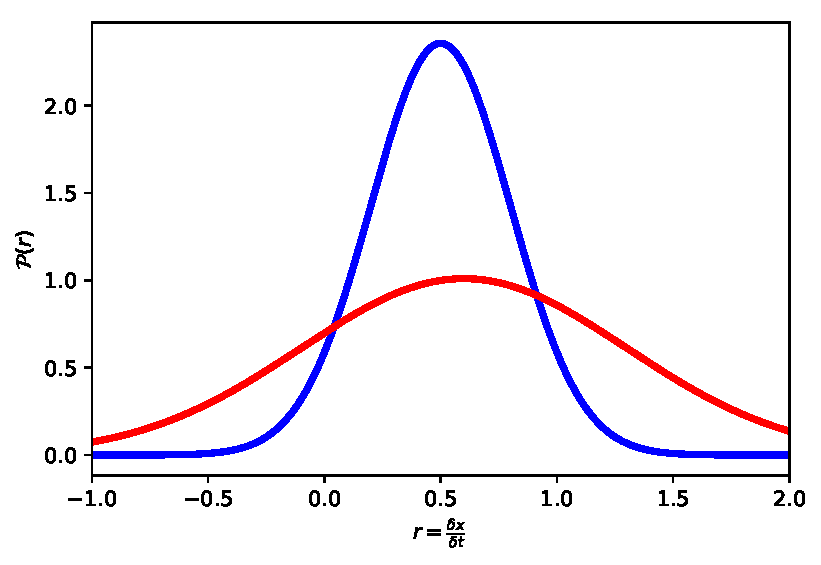
\includegraphics[width=\textwidth]{./chapter_riskless/figs/two_dists.pdf}
%\caption{Two possible probability density functions for the per-round 
%multiplier, $\gr$, defined in \eref{R_def}. The distribution denoted by 
%the blue line has a higher mean and a higher variance than the one 
%in red. How are we to decide which represents the more favourable 
%gamble?\flabel{dec_dist}}
%\end{figure}



\section{Decisions in a deterministic world}
\seclabel{Decisions_in_a_deterministic}
\subsection{Different magnitudes}
I'm off to the bank to withdraw some money for you. I offer to give you either
\bi
\item[(1)] \$20 when I 
get back or 
\item[(2)] \$50 when I get back. You tell me what you prefer.
\ei
Let's see what our decision axiom says you'll do. Remember there's no uncertainty, I'm not lying to you, no one will rob me on my way from the bank \etc

I haven't told you how long it will take me to get to the bank, so let's keep that general and call that time interval $\Dt$.
Because we know that $\Dt$ is the same under options (1) and (2) we don't actually need to know its value to compare the growth rates for the two options. 
We don't even have to know much about the functional form of the growth rate - we know that different situations require different forms of growth rates. 
In the present case it turns out that any growth rate will give the same answer. Let's see.
Under option a) we have
\be
\g^{(1)} =\frac{\gv(\x+\$20)-\gv(\x)}{\Dt},
\ee
and under option b) we have
\be
\g^{(2)} =\frac{\gv(\x+\$50)-\gv(\x)}{\Dt}.
\ee
To find out which growth rate is larger, we subtract $\g^{(a)}$ from $\g^{(b)}$ 
\bea
\g^{(2)}-\g^{(1)} &=&\frac{\gv(\x+\$50)-\gv(\x)(-\gv(\x+\$20)-\gv(\x))}{\Dt}\\
 &=&\frac{\gv(\x+\$50)-\gv(\x+\$20)}{\Dt}.
\eea
Because $\gv(\x)$ is monotonically increasing, any growth rate will be greater under option (2), and 
our model humans will always go for option (2). That's good -- because I would have chosen option (2) if I were you, and 
our model reproduces this intuitive result.

More generally, our model says: of two certain payments of different sizes at the same time, choose the bigger one.

\subsection{Different magnitudes and times - discounting}
\seclabel{Different_magnitudes_and}
Let's make the decision a little harder: what if I offer you 
\bi
\item[(1)] \$10 in a month or 
\item[(2)] \$25 in two months?
\ei
Again, we will compute the two growth rates corresponding to options (1) and (2), and then choose the bigger one -- that's how we have been programmed to behave in the world that our axiom is creating. But unlike in the previous case, the functional form of the growth rate will now be important. 

Let's start with the exponential growth rate, with $\gv(\x)=\ln \x$ in \eref{gen_rate} -- this is the appropriate rate if wealth grows exponentially, like in a savings account.
We now have growth rates
\be
\gm^{(1)} =\frac{\ln(\x+\$10)-\ln(\x)}{1 \text{ month}},
\ee
and
\be
\gm^{(2)} =\frac{\ln(\x+\$25)-\ln(\x)}{2 \text{ months}}.
\ee
Curiously, which is greater depends on your initial wealth, in our model world. If your wealth is \$100, then $\gm^{(1)}\approx 114\%$ p.a., and 
$\gm^{(2)}\approx 134\%$ p.a., wherefore you will choose option (2).

But if your initial wealth is \$1, then $\gm^{(1)}\approx 2,877\%$ p.a. and $\gm^{(2)}\approx 1,955\%$ p.a., and you'll choose option (1).

We learn: in this slightly more complex though still fully deterministic case, which option is 
preferable does not only depend on the options available but also on the personal 
circumstances (initial wealth) of the decision maker.

\begin{figure}
\centering
\begin{picture}(200,80)(0,0)
 \put(-75,0){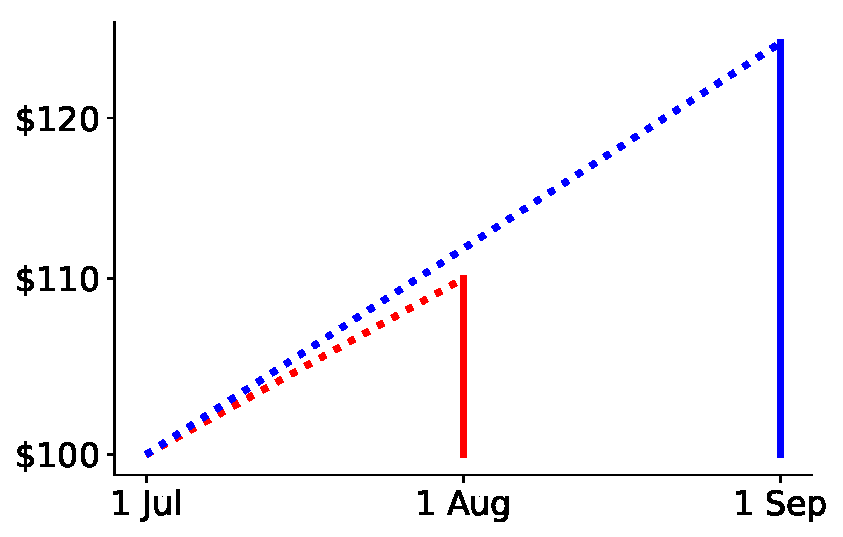
\includegraphics[width=.45\textwidth]{./chapter_riskless/figs/exp_disc_2.pdf}}
 \put(120,0){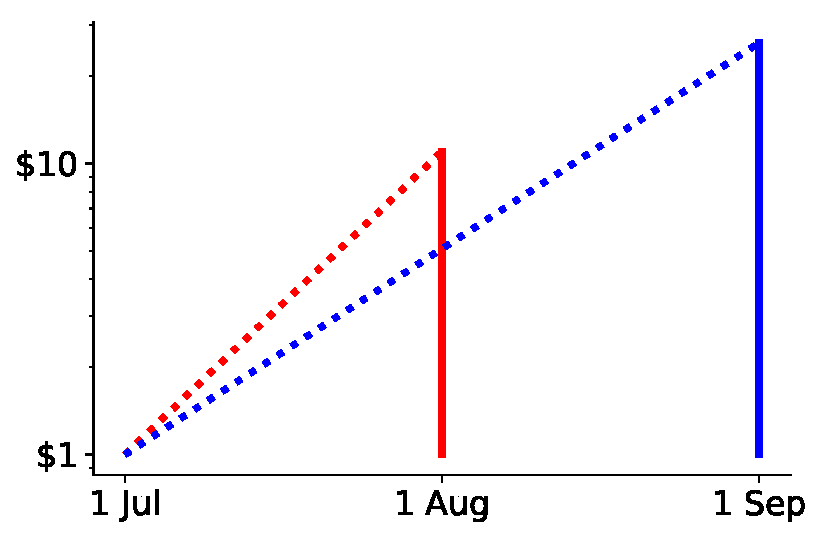
\includegraphics[width=.45\textwidth, angle=0]{./chapter_riskless/figs/exp_disc_1.pdf}}
 \put(-35,80){A}
 \put(155,80){B}
\end{picture}
\caption{\small Slopes with logarithmic vertical scales. (A) If you have a lot of money (here \$100), exponential growth-rate optimization tells you to be patient and choose the later, larger, payment of \$25. (B) If you have little money (here \$1), the same criterion -- exponential growth-rate optimization -- tells you to get the cash as fast as possible, and choose the earlier, smaller, payment of \$10.}
\flabel{hyp_disc}
\end{figure}


Notice how the poorer decision maker seems to be more impatient, despite his use of the exact same decision axiom.
Using $\gv(\x)=\ln(\x)$ in \eref{} is related to what's called ``exponential discounting'' in the economics literature \cite{MavroyiannisETAL2019}.

What about the additive growth rate? That would be the relevant growth rate to compute if, for instance, these payments to us are promised as a salary. I already know what you'd pick: \$1 per month, or \$3 per two months? The reason I know what you'd choose is that it doesn't depend on your initial wealth. Let's see, that's just working with the identity function $\gv(\x)=\x$ in \eref{gen_rate}.
\be
\gad^{(1)} =\frac{\x+\$1-\x}{1 \text{ month}} \approx \$0.083 \text{ p.a.},
\ee
and
\be
\gad^{(2)} =\frac{\x+\$3-\x}{2 \text{ months}}\approx \$0.167 \text{ p.a.}.
\ee
Initial wealth cancels out: this is a unique feature of the additive growth rate. Only under additive dynamics does initial wealth not enter into the computation of the growth rate, and growth rates can be computed with knowledge of only the payouts and waiting times.

In the economics literature, decision-making based on additive growth rates is called ``hyperbolic discounting'' because this case is mathematically equivalent to discounting payments in the future with the hyperbolic function $\frac{1}{\Dt}$.

An interesting feature of optimizing additive growth rates is what's called ``preference reversal:'' let's keep our example as it is, except we now let time march forward, holding fixed the moments in time when the payments are to be made. Under these conditions, there comes a time, precisely after half a month, when option (2) is no longer preferred, see \fref{hyp_disc}.

\begin{figure}
\centering
\begin{picture}(200,80)(0,0)
 \put(-80,0){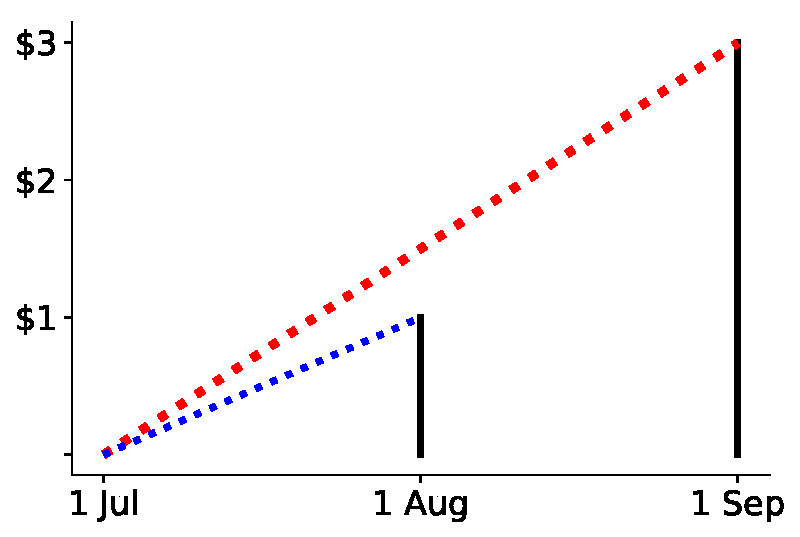
\includegraphics[width=.33\textwidth]{./chapter_riskless/figs/disc_1.pdf}}
 \put(40,0){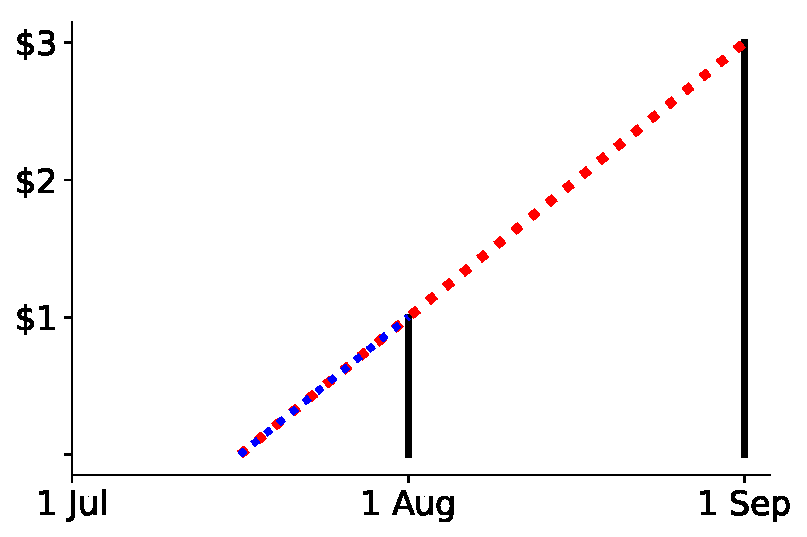
\includegraphics[width=.33\textwidth, angle=0]{./chapter_riskless/figs/disc_2.pdf}}
 \put(160,0){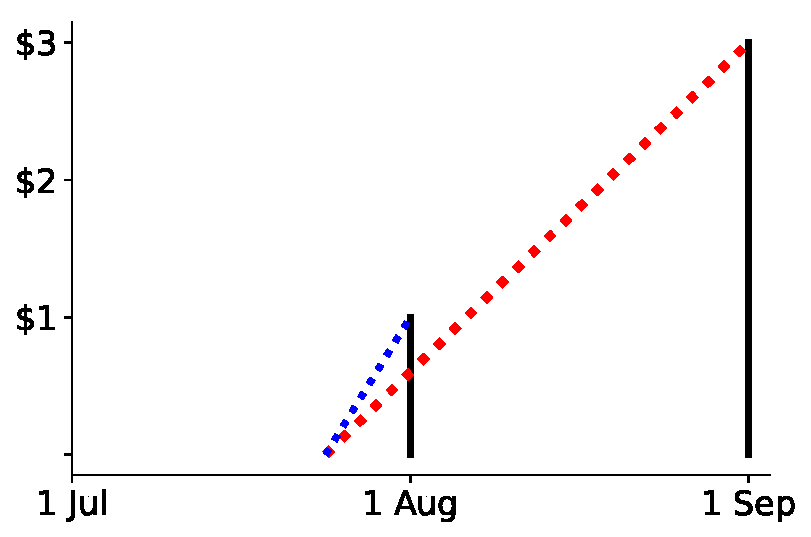
\includegraphics[width=.33\textwidth, angle=0]{./chapter_riskless/figs/disc_3.pdf}}
\put(-60,60){A}
\put(60,60){B}
\put(180,60){C}
\end{picture}
\caption{\small  Slopes with linear vertical scales. (A) At the beginning option (2) yields the highest additive growth rate; (B) after half a month, the options are equally good; (C) after 3/4 of a month, preference reversal has taken place, and option (1) now yields the highest growth rate. As the first payment approaches, the associated growth rate diverges.}
\flabel{hyp_disc}
\end{figure}

Perhaps the most significant message is the richness of this problem. We're applying nothing but our simple axiom, but it forces us to choose how we think about the dynamics of our wealth, and in reality that may depend strongly on many difficult to specify circumstances. In real life payments are not just offered at some point in time, but usually in return for something -- an asset or work. Depending on the specific exchange, an additive, multiplicative, or more general model will be appropriate.

Importantly, we need not resort to psychology to generate a host of behaviours, such as impatience of poorer individuals or preference reversal as time ticks on.


%%%%%%%%%%%%%%%%%%%%%%%%%%%%%%%%%%%%%%%%%%%%%%%
\section{The St Petersburg paradox}
The problem known today as the St Petersburg paradox was suggested by Nicolaus 
Bernoulli\footnote{Daniel's cousin. The Bernoulli family produced a remarkable 
number of famous mathematicians in the $17^\text{th}$ and $18^\text{th}$ centuries, 
who helped lay the foundations of applied mathematics and physics.} in 1713 in his 
correspondence with Montmort~\cite{Montmort1713}. It involves a hypothetical 
lottery for which the rate of change of expected wealth diverges for any finite ticket 
price. The expected-wealth paradigm would predict, therefore, that people are 
prepared to pay any price to enter the lottery. However, when the question is put 
to them, they rarely want to wager more than a few dollars. This 
is the paradox. It is the first well-documented example of the inadequacy of the 
expected-wealth paradigm as a model of human rationality. It was the primary 
motivating example for Daniel Bernoulli's and Cramer's development of the 
expected-utility paradigm~\cite{Bernoulli1738}.

In some sense it is a pity that this deliberately provocative and unrealistic lottery has played such an important role in the development of classical decision theory. It is quite unnecessary to invent a gamble with a diverging change in expected wealth to expose the flaws in the expected-wealth paradigm. The presence of infinities in the problem and its variously proposed solutions has caused much confusion, and permits objections on the grounds of physical impossibility. Such objections are unhelpful because they are not fundamental: they address only the gamble and not the decision paradigm. Nevertheless, the paradox is an indelible part not only of history but also of the current debate~\cite{Peters2011b}, and so we recount it here. We'll start by defining the lottery.

\begin{example}{St Petersburg lottery}
The classical statement of the lottery is to imagine a starting prize 
of $\$1$ (originally the prize was in ducats). A fair coin is tossed: 
if it lands heads, the player wins the prize and the lottery ends; if it lands 
tails, the prize is doubled and the process is repeated. Therefore, the 
player wins $\$2$, $\$4$, $\$8$ if the first head lands 
on the second, third, fourth toss, and so on. The player must buy a ticket, 
at price $\F$, to enter the lottery. The question usually posed is: what is 
the largest $\F$ the player is willing to pay?

The lottery can be translated neatly into our gamble formalism:
\be
\q_\gj = \$ 2^{\gj-1} - \F, \quad \p_\gj = 2^{-\gj},
\elabel{lottery_def}
\ee
for $\gj\in\{1,2,3,\ldots\}$, \ie the set of positive integers. The vast majority 
of observed payouts are small, but occasionally an extremely large payout 
(corresponding to a very long unbroken sequence of tails in the classical 
description) occurs. This is shown in the example trajectories in 
\fref{lottery_add_traj}, where the lottery has been repeated additively.

From now on we will forget about the coin tosses, which are simply a 
mechanism for selecting one of the possible payouts. In effect, they 
are just a random number generator. Instead we shall work with the 
compact definition of the lottery in \eref{lottery_def} and assume it 
takes a fixed amount of time, $\dt$, to play.

The rate of change of expected wealth is
\bea
\frac{\ave{\d\x}}{\dt} & = & \frac{1}{\dt} \sum_{\gj=1}^\infty \p_\gj \q_\gj \\
&=& \frac{1}{\dt} \left( \$ \sum_{\gj=1}^\infty 2^{-\gj}\,2^{\gj-1} - \sum_{\gj=1}^\infty 2^{-\gj} \F \right) \\
&=& \frac{1}{\dt} \left( \$ \sum_{\gj=1}^\infty \frac{1}{2} - \F \right). \elabel{lottery_ex_wealth}
\eea
This diverges for any finite ticket price. Under the expected-wealth paradigm, this means that the lottery is favourable at any price.
\end{example}
\begin{figure}
\centering
\begin{picture}(200,230)(0,0)
\put(-75,0){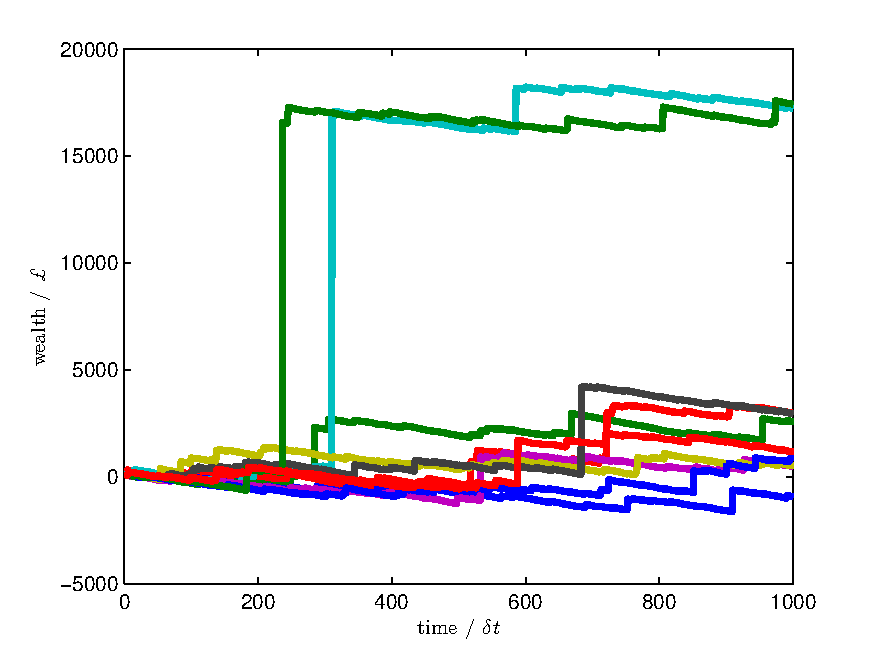
\includegraphics[width=\textwidth]{./chapter_riskless/figs/lottery_add_traj.pdf}}
\end{picture}
\caption{Wealth trajectories for the additively repeated St Petersburg lottery, 
with starting wealth, $\x(0)=\$100$, and ticket price, $\F=\$10$. 
Ten trajectories are plotted over 1,000 rounds.\flabel{lottery_add_traj}}
\end{figure}

This implausible conclusion, which does not accord with human behaviour, 
exposes the weakness of judging a gamble by its effect on expected 
wealth. Daniel Bernoulli suggested to resolve the paradox by adopting 
the expected-utility paradigm. His choice of utility function was the 
logarithm, $\gu(\x)=\ln \x$, which, as we now know, produces a decision 
rule equivalent to growth-rate optimisation under multiplicative repetition. 
This correspondence was not appreciated by Bernoulli: indeed $18^\text{th}$-century mathematics did not possesse the concepts and 
language required to distinguish between averages over time and across 
systems, even though it had the basic arithmetic tools. 
%In any case, the 
%correspondence relies on the choice of a particular utility function, and vanishes the moment something other than the logarithm is chosen. We also have
%to interpret expected utility theory a little differently from how it is usually presented -- for instance we have to assume that expected changes in utility really mean expected rates of changes, with a specific gamble duration, \ie we have to introduce the concept of time into utility theory quite differently from that's usually done (which we won't discuss here).

Unfortunately, Bernoulli made a mathematical error in the implementation 
of his own paradigm -- accidentally he proposed two mutually inconsistent versions of utility theory in the paper that established the paradigm. Initially, the error had little impact, and it was corrected by Laplace in 
1814~\cite{Laplace1814}. But Laplace didn't openly say he'd corrected an error, he just worked with what he thought Bernoulli had meant. This politeness had awful consequences. In
1934 Menger~\cite{Menger1934}, keen to get the story right, went back to the original text by Bernoulli. He didn't notice the error but rather got confused by it which led him to introduce a further error. Based on this car crash of scientific communication, Menger derived the infamous (wrong) claim we encountered in \secref{Technical}: utility functions must be bounded, with disastrous consequences for the budding neoclassical formalism. We 
will leave this most chequered part of the paradox's history alone -- details can be found 
in~\cite{PetersGell-Mann2016}. Instead we will focus on what's usually 
presumed Bernoulli meant to write.

\begin{example}{Resolution by logarithmic utility}
Instead of \eref{lottery_ex_wealth}, we calculate the rate of change of expected logarithmic utility,
\bea
\frac{\ave{\d\ln \x}}{\dt} & = & \frac{1}{\dt} \sum_{\gj=1}^\infty \p_\gj \left[\ln(\x+\q_\gj)-\ln \x\right] \\
&=& \frac{1}{\dt} \sum_{\gj=1}^\infty 2^{-\gj} \ln\left(\frac{\x+\$2^{\gj-1}-\F}{\x}\right), \elabel{lottery_ex_util}
\eea
where $\x$ is the ticket buyer's wealth.

This is finite for all finite ticket prices less than the buyer's wealth plus the smallest 
prize: $\F<\x+\$1$. This can be shown by applying the ratio 
test.\footnotemark\ It may be positive or negative, depending on the values 
of $\F$ and $\x$. \fref{gbar_zero} shows the locus of points in the $(\x,\F)$-plane 
for which the sum is zero.
\end{example}
\footnotetext{The ratio of the $(\gj+1)^\text{th}$ term to the $\gj^\text{th}$ term 
in the sum tends to $1/2$ as $\gj\to\infty$.}
\begin{figure}
\centering
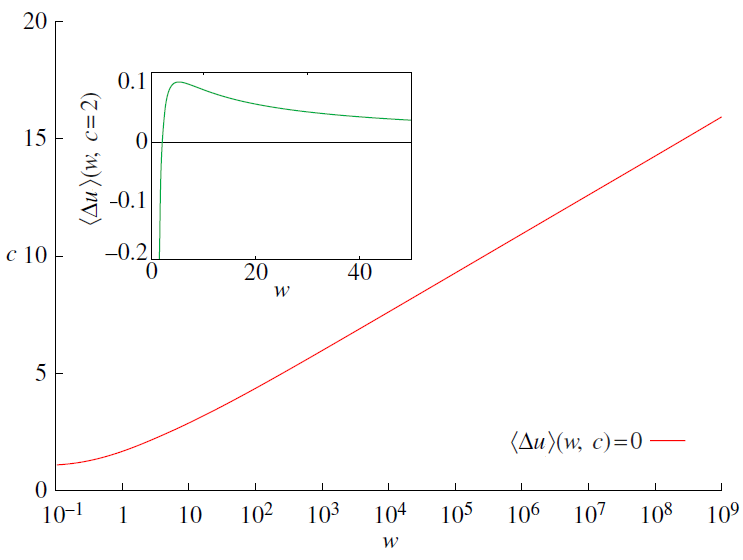
\includegraphics[width=\textwidth]{./chapter_riskless/figs/gbar_zero.png}
\caption{Locus of points in the $(\x,\F)$-plane for which the expected change in 
logarithmic utility is zero. The inset shows the expected change in utility as a 
function of $\x$ for $\F=\$2$. Adapted from~\cite{Peters2011b}.\flabel{gbar_zero}}
\end{figure}

The utility paradigm is a model that resolves the paradox, in the sense that creates a world where players may decline to buy a ticket. Bernoulli argued for this resolution framework in plausible terms: the usefulness of a monetary gain depends on how much money you already have. He also argued specifically for the logarithm in plausible terms: the gain in usefulness should be proportional to the fractional gain it represents, $\d \gu = \d\x/\x$. Yet, the framework has left many unsatisfied: why does usefulness have this functional form? We provide this deeper reason by connecting the problem to dynamics and time, unlike Bernoulli. Had Bernoulli made the connection, he might have been less willing to accept Cramer's square-root utility function as an alternative, which, as we've seen, corresponds to a rather less intuitive dynamic.

%However, while plausible, the framework relies on a utility function, which must be postulated. It can neither be derived from fundamental considerations nor verified empirically.

Turning to our decision algorithm, we will assume that the lottery is repeated multiplicatively. This means, in effect, that the prizes and ticket price are treated as fractions of the player's wealth, such that the effect of each lottery is to multiply current wealth by a random factor,
\be
\gr_\gj = \frac{\x+\$2^{\gj-1}-\F}{\x}, \quad \p_\gj= 2^{-\gj}.
\ee
This follows precisely our earlier treatment of a gamble with multiplicative dynamics, and we can apply our results directly. 
The time-average (exponential) growth rate is
\be
\gt_\text{m} = \frac{1}{\dt} \lim_{\T\to\infty} \left\{ \frac{1}{\T}  \sum_{\gtau=1}^\T \ln \gr(\gtau) \right\} = \frac{1}{\dt}  \sum_{\gj=1}^\infty 2^{-\gj} \ln \gr_\gj, \elabel{lottery_gbar}
\ee
which is identical to the expression for the rate of change of expected log-utility, 
\eref{lottery_ex_util}. This is, as we've discussed, because $\gv(\x)=\ln(\x)$ 
is the appropriate ergodicity mapping for multiplicative dynamics. The result is the same, but 
the interpretation is different: we have assumed less, only that our player is 
interested in the growth rate of his wealth and that he gauges this by imagining 
the outcome of an indefinite sequence of repeated lotteries.

Thus the locus in \fref{gbar_zero} also marks the decision threshold \textit{versus} 
the null gamble under our decision axiom. The player can sensibly decline the 
gamble, even though it results in a divergent change in expected wealth. This 
is illustrated by comparing \fref{lottery_mult_traj}, which shows trajectories of 
multiplicatively repeated lotteries, with the additively repeated lotteries already 
seen in \fref{lottery_add_traj}.
\begin{figure}
\centering
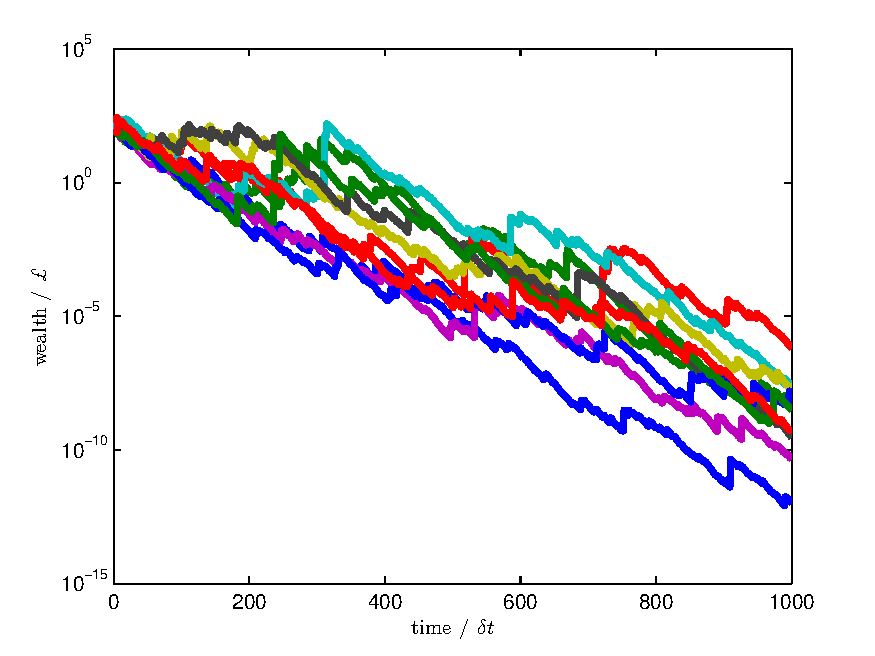
\includegraphics[width=\textwidth]{./chapter_riskless/figs/lottery_mult_traj.pdf}
\caption{Wealth trajectories for the multiplicatively repeated St Petersburg lottery, 
with starting wealth, $\x(0)=\$100$, and ticket price, $\F=\$10$. Ten 
trajectories are plotted over 1,000 rounds. The realisations of the individual 
lotteries are the same as in \fref{lottery_add_traj} but the mode of repetition is 
different.\flabel{lottery_mult_traj}}
\end{figure}
The trajectories are based on the same sequences of lottery outcomes, only 
the mode of repetition is different. The simulation shows us visually what we 
have already gleaned by analysis: what appears favourable in the 
expected-wealth paradigm (corresponding to additive repetition) results in a 
disastrous decay of the player's wealth over time under a realistic dynamic.

As $\F\to \x+\$1$ from above in \eref{lottery_gbar}, $\gt_\text{m}$ diverges 
negatively, since the first term in the sum is the logarithm of a quantity approaching 
zero. This corresponds to a lottery which can make the player bankrupt. The effect 
is also shown in the inset of \fref{gbar_zero}.

Treatments based on multiplicative repetition have appeared sporadically in the 
literature, starting with Whitworth in 
1870~\cite[App.~IV]{Whitworth1870}.\footnote{Whitworth was dismissive of early utility theory: ``The result at which we have arrived is not to be classed with 
the arbitrary methods which have been again and again propounded to evade the difficulty of the Petersburg problem\ldots. Formulae have often been proposed, which have possessed the one virtue of presenting a finite result\ldots but they have often had no intelligible basis to rest upon, or\ldots sufficient care has not been taken to draw a distinguishing line between the significance of the result obtained, and the different result arrived at when the mathematical expectation is calculated.'' Sadly he chose to place these revolutionary remarks in an appendix of a college probability textbook.} It is related to the famous Kelly Criterion~\cite{Kelly1956}\footnote{Kelly was similarly unimpressed with the mainstream and noted in his treatment of decision theory, which he developed from the perspective of information theory and which is identical to ergodicity economics with multiplicative dynamics, that the utility function is ``too general to shed any light on the specific problems of communication theory.''}, although Kelly did not explicitly treat the St Petersburg game, and tangentially to \Ito's lemma~\cite{Ito1944}. It appears as an exercise in a well-known text on information theory~\cite[Ex.~6.17]{CoverThomas1991}. Mainstream economics has ignored all this. A full and rigorous resolution of the paradox, including the epistemological significance of the shift from ensemble to time averages, was published recently by one of the present authors~\cite{Peters2011b}.
